\documentclass{article}
\usepackage[english]{babel}
\usepackage{fullpage}
\usepackage{graphicx}
\usepackage{enumitem}
\usepackage{url}
\usepackage[usenames, dvipsnames]{color}
\usepackage[utf8]{inputenc}
\usepackage{footmisc}

\title{\textbf{CSE 564 Project Report (Draft)} 
\\
\begin{center}
\LARGE{Is Your Smart Home Secure?}
\end{center}\vspace{-2ex}}
\author{Jeanette Daum (jdaum), Chandrakana Nandi (cnandi) }
\date{March 3, 2016}

\begin{document}

\maketitle
\begin{abstract}
One of the applications of Internet of Things which is gaining popularity is Home Automation. These systems are typically made up of devices which can be controlled remotely by the home inhabitants or can communicate with each other and act autonomously. An objective for smart homes is ensuring their security and correctness because violation of these properties can directly affect the lives of the inhabitants. What if the controller of one device incorrectly sends commands to another device or sends the command to a device under incorrect conditions? In this project, we design and implement an abstract architecture for modelling smart homes in a way that makes it easier to reason about their security and correctness, define different types of policies and specify them for three different smart systems and develop a static analyzer that verifies whether the implementation of the smart systems complies with the specified policies. 

\end{abstract}
\section{Introduction}
Home automation systems are a new trend that is just starting to gain momentum and will soon have a huge impact on our everyday lives~\cite{samsung, homekit, echo, wink, homeos}. Typically, these systems consist of devices interacting with each other. These devices can take actions autonomously or they can be controlled remotely by the home inhabitants. An example is a garage door that opens automatically whenever the car is within a certain distance, but also opens and closes when the user gives a remote command by pressing a button. 

For our project, we consider a smart home to be a collection of interacting devices acting autonomously without requiring the user to intervene. Nowadays most of the existing systems require user interaction and remote control but we expect future systems to become more autonomous to further assist its inhabitants~\cite{homekit}.

A challenge for smart homes is to ensure that there are no security loopholes because they can be exploited by malicious attackers to take control of the house and harm the inhabitants~\cite{yoshi, jung}. For autonomous systems, security and correctness is even more crucial because the user relies on the system and may not have much control over it. Before smart homes become as widespread as smart phones are today, it is necessary for the home automation industry to address these concerns.

In this project, our goal is to ensure that a system of interacting smart devices satisfies a set of security properties. We are concerned with security at the device level and not with the security of the communication protocols or the underlying operating system. We aim to solve the problem of security for smart homes from the point of view of the manufacturers of the smart devices so that they can guarantee that their devices are trustworthy, and the major smart home platform providers such as Samsung and Apple so that they can guarantee that they only integrate secure and correct devices to their platform. Section~\S\ref{subsec:roles} describes the roles played by manufacturers of devices, users and platform providers (such as Samsung, Apple, etc.) in our model in detail.

We have modelled a smart home as a collection of three types of devices: controllers, sensors and dumb-devices. The controllers send commands to the dumb-devices based on values of sensors which measure different parameters such as temperature, state of a dumb-device, etc. The dumb-devices simply execute the commands sent to them.
We defined a set of security policies and specified them for three different smart systems: a smart laundry system, a smart garage door system and an HVAC system. We developed a static analyzer that verifies that the three smart systems adhere to their respective policies. By conducting a preliminary experiment explained in section~\S\ref{sec:analysis}, we show that for smart homes, dynamically enforcing security policies can lead to a large overhead which may affect the reliability of the system. This motivates our decision of doing static program verification to provide compile time guarantees that a smart home is secure. Our main contributions are:
\begin{itemize}[topsep=0pt,itemsep=0ex,partopsep=1ex,parsep=1ex]
    \item Designing a smart home architecture, implementing a prototype of the architecture and three smart systems based on it; a smart laundry system, a smart garage door, and an HVAC system.    
    \item Defining and formalizing different types of security and correctness policies and specifying one of them for the three smart systems.
    \item Developing a static analysis tool for verifying the code of the smart systems.
    \item Analysing the roles played by different organizations/individuals in the smart home business and proposing a model for distributing the tasks of specification, implementation and verification among them.
\end{itemize}
  
\section{Related work}
Some researchers have suggested general solutions for ensuring security for smart homes such as choosing a stronger password for protecting the devices or modifying their security settings according to one's needs~\cite{semantec}. Such solutions rely on the user's awareness about security vulnerabilities and do not address the problems specific to smart homes such as devices with different functionalities interacting without user intervention. Hence they cannot guarantee that a smart home will always behave correctly. Another proposed solution~\cite{al2000secure} is based on dynamic enforcement. The problem with dynamic solutions is that if a security breach is encountered during execution, the service has to be stopped. This is not convenient from the user's point of view because it affects the reliability of the system. Further, as we show in section~\S\ref{sec:analysis}, enforcing security and correctness policies dynamically leads to an execution time overhead which is not desirable in home automation. Consider a situation where there is a fire in the house and the inhabitants want to evacuate as soon as possible. If there is dynamic policy checking, that might cause delay in the opening of the front door which can affect the physical safety of the people. 
In this paper, our idea is to specify security and correctness policies for the smart devices in a home and verify them statically thereby providing compile time guarantees that the entire smart home is secure and correct. In section~\S\ref{subsec:roles}, we describe in detail who is responsible for doing the verification according to our proposed model.

\section{Architecture and stakeholders}
\label{sec:archi}
We present a high-level modular architecture for designing smart homes which classifies devices into three categories depending on their functionality: \textit{sensors}, \textit{controllers} and \textit{dumb devices}. There are two types of messages exchanged among the devices: 
\begin{itemize}[topsep=0pt,itemsep=-1ex,partopsep=1ex,parsep=1ex]
    \item \textit{informational}: Sensors broadcast information such as the state of a dumb device or the temperature in the house.  
    \item \textit{commands}: Controllers send commands to the dumb devices telling them what to do. A command has two components, an action part and a dumb device part and is represented as:   \texttt{action\_dumbdevice}. The former represents what the receiving dumb device must do and the latter represents the type of dumb device that can execute the command.
\end{itemize}

\begin{figure}
\begin{center}
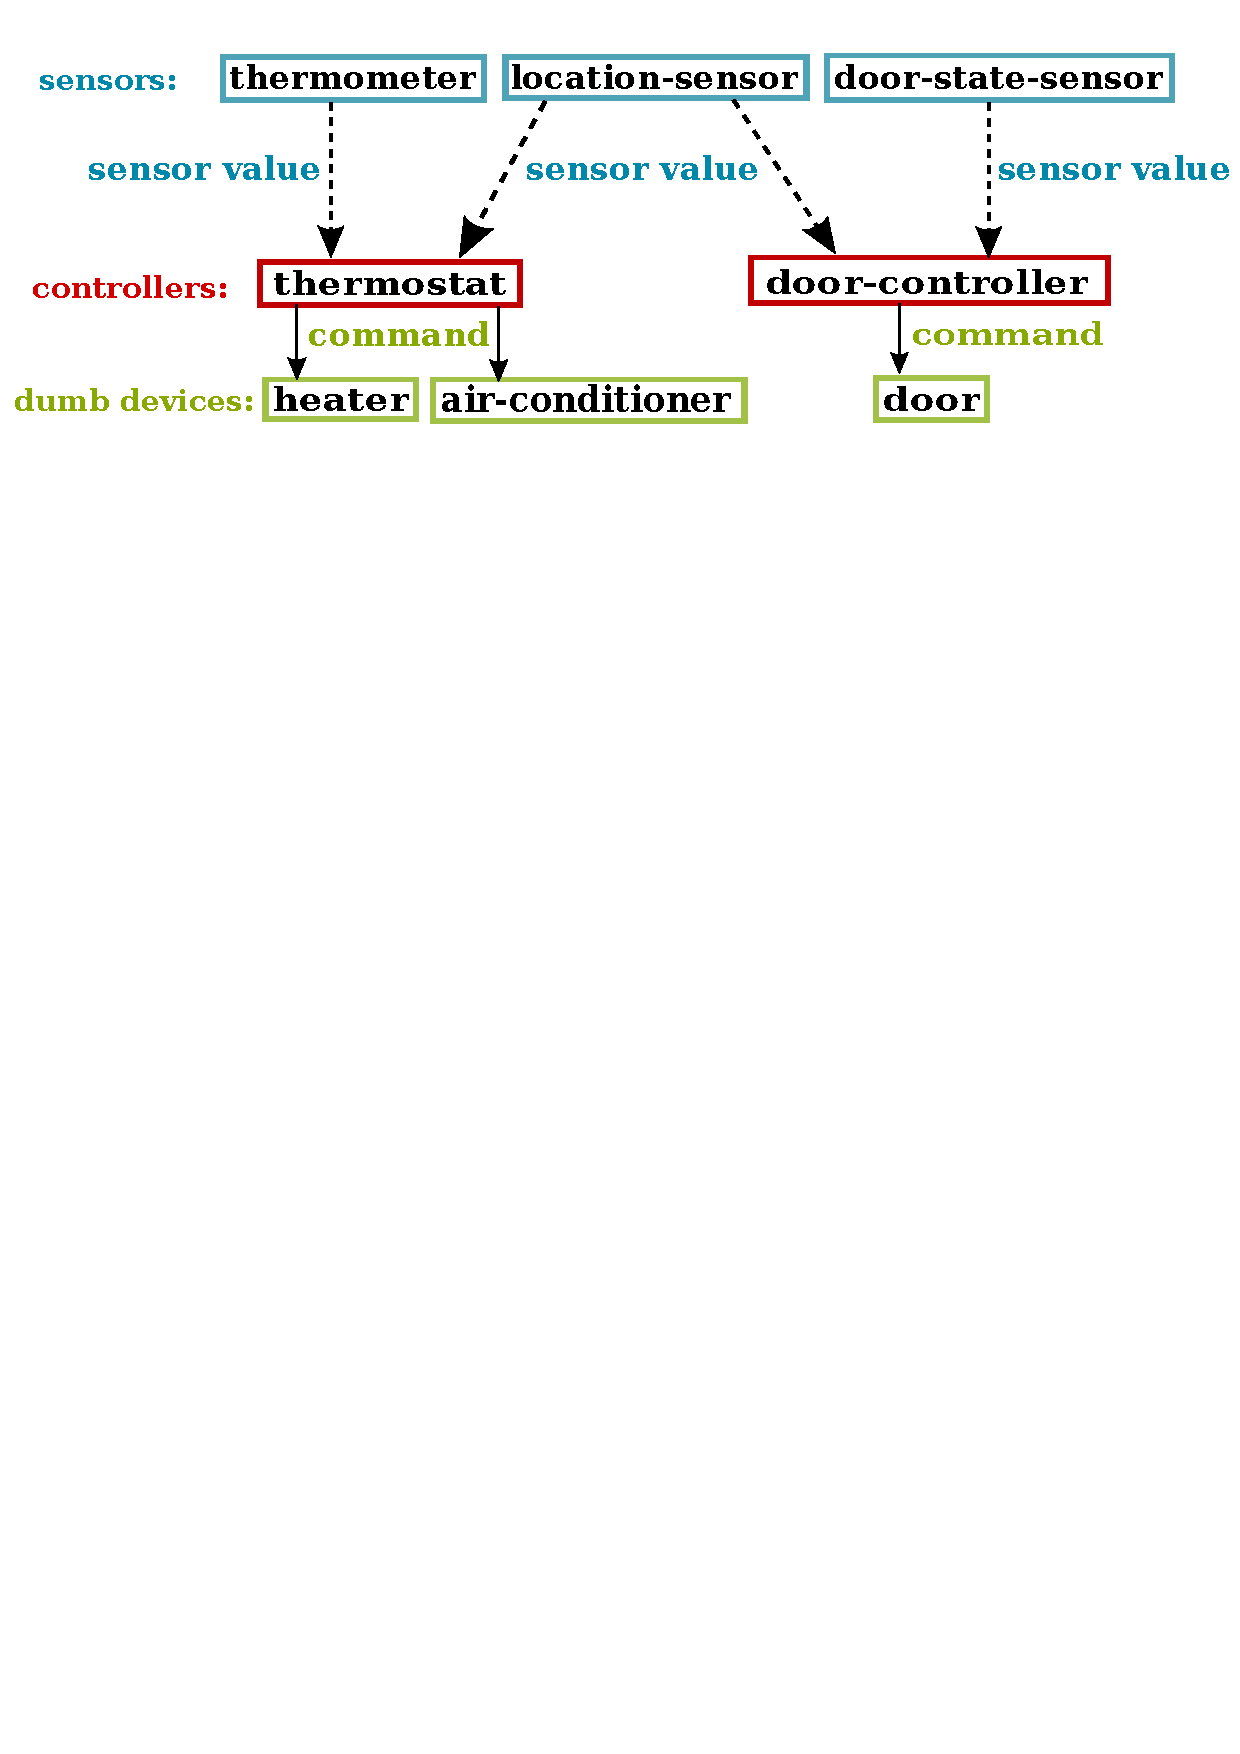
\includegraphics[scale=0.4, trim= 0 600 0 0]{figure1.pdf}
\caption{\color{RoyalBlue}{Sensors}, \color{Maroon}{controllers,} \color{black}{and} \color{LimeGreen}{dumb devices}. %\color{black}{The thermostat sends commands depending on values from two sensors: the thermometer and the location sensor. The door controller also sends commands depending on the values of two sensors: the location sensor and the current state of the door.}
}
\label{fig:arch}
\end{center}
\end{figure}

\subsection{Sensors, controllers and dumb devices}
\label{subsec:devices}
\textit{Sensors} measure properties like temperature, motion, state of a dumb device, etc. and notify controllers depending on them. Sensors can be inside or outside the house. Examples of sensors inside the house are: motion detectors, the thermostat etc. and outside the house are: a camera outside the main door or the GPS sensor in the owner's smart phone when the owner is outside. 

\textit{Controllers} send commands directly to some of the dumb devices depending on the values of one or more sensors. 
%They have a set of commands they can send and a set of \textit{dependency policies} which specify the conditions (sensor values) under which they can send a command to a dumb device. Both of these are the specifications against which a controller's implementation is verified. 

%A dumb device %belongs to some category such as room-heater, air-conditioner, light-bulb, garage-door etc. and 
%has a set of actions it can execute, such as on, off, open, close etc. 
\textit{Dumb devices} do not send messages to other dumb devices, sensors, or controllers. They atomically execute the commands sent to them by any controller. 

It is not necessary for the sensors, controllers, and dumb devices to be physically separate from each other: 
a controller may be fit to a dumb device or a dumb device may have sensors attached to it. For formal reasoning about the system, we treat them as separate entities. Figure~\ref{fig:arch} illustrates the architecture of a simple example smart system. 

In our high-level architecture, we abstract away the lower level details of a smart home such as the underlying communication protocols and focus on the different devices.

\subsection{Roles of different organizations}
\label{subsec:roles}
We consider the entire smart home business to comprise of four different groups playing different roles. We propose a hierarchical certification mechanism to ensure that smart homes satisfy certain security and correctness standards (similar to the app store model). The  mechanism is hierarchical so that it can scale to a very large number of manufacturers who are interested in developing smart devices.   
\begin{itemize}[topsep=0pt,itemsep=0ex,partopsep=1ex,parsep=1ex]
\item \textit{Watchdog organizations}: Similar to standards like IEEE and IEC, we propose organizations to be developed for specifying certain standards for smart homes. The organizations would define security, privacy and correctness specifications which should ideally be met by all smart devices. An example specification related to information flow could be that information from within the smart home should not be sent to the cloud without user permission. Another example of a specification related to access control could be that the controller of a certain category of devices may not control devices which do not fall in that category (a garage door and a coffee maker would not be in the same category). Yet another example of a specification related to sensor dependency could be that a controller may send a command only under certain sensor conditions.
\item \textit{Platform providers}: We define platform providers as companies such as Samsung~\cite{samsung}, Apple~\cite{homekit}, etc. who provide platforms (hubs or apps) for integrating different smart devices and communication protocols to make them interact with each other or allow the users to control them remotely. In our model, we consider these organizations to have their own methodology for specifying the standards defined by the \textit{watchdog organizations} and verifying devices against them. For example the methodology could be a domain specific language for specifying the policies and a type system for verifying them. 
These organizations would be inspected by the \textit{watchdog organizations} and marked as ``certified" if the \textit{watchdog organizations} find that their mechanisms for specifying and verifying the standards are acceptable.


\item \textit{Third-party device manufacturers}: They are the companies like Philips, Withings and numerous other small manufacturers who develop \textit{controllers}, \textit{dumb-devices} and \textit{sensors}~\cite{workswithsmartthings, workswithhomekit} which can be integrated to the platforms developed by the \textit{platform providers}. The latter themselves can also be device manufacturers; both Samsung and Apple manufacture their own smart devices. 
The \textit{platform providers} would release APIs for implementing devices which can be used by third-party device manufacturers so that their products can be integrated to the platforms of the former.
Before  allowing any device manufactured by a third party to be integrated to their platform, the platform providers must verify the code against the specifications. The devices that pass the verification would be marked as ``certified" and may be trusted. 

\item \textit{End users}: They are the home inhabitants who own (or want to own) a smart home. An end user might want to buy a hub (or app) from one of the existing \textit{platform providers} to plug in different smart devices bought either from the \textit{platform providers} or from some \textit{third-party device manufacturer} and convert their ordinary home to a smart home. As long as the devices are marked as ``certified" by one of the \textit{platform providers}, the end user can trust them due to the hierarchical certification mechanism.
\end{itemize}



%Verification of the policies we defined ensures that (a) a controller does not send commands to a dumb device it owns under the wrong conditions, (b) it only send correct commands to the correct dumb devices, and (c) adding a new device to the house does not violate any security or correctness policy. \\

%\subsection{Device discovery}
%\label{subsec:discovery}
%A controller can discover other controllers, sensors, and dumb devices and the commands the latter can execute. If these commands match with the commands the controller can send, then it can take charge of the dumb device. Every controller stores a table mapping the IDs of the controllers to a list of pairs of dumb device IDs and commands the controllers may send to them. Two example entries are:\\
%\{\texttt{thermostatID:\{(roomheaterID, start\_roomheater), \\ 
%\hspace*{2.5cm}(roomheaterID, stop\_roomheater),\\ 
%\hspace*{2.5cm}(airconditionerID, start\_airconditioner), \\
%\hspace*{2.5cm}(airconditionerID, stop\_airconditioner)\}\\
%\hspace*{0.2cm}doorcontrollerID:\{(doorID, open\_door),\\
%\hspace*{3.0cm} (doorID, close\_door)\}\}
%}\\

%\noindent The controllers stay in sync with identical contents in their tables. If there is no controller that can send the commands a dumb device can execute, no message will be sent to it unless a suitable controller for it is installed. %When this new controller is installed, it discovers all the other dumb devices, sensors and controllers in the house (and is likewise discovered by all the existing controllers). It updates its table with the entries from all the other controllers and adds the dumb device with the corresponding commands against its ID in the table, after which the tables of all the other controllers are updated. 
%Once a dumb device and a command it can execute are chosen by a controller, no other controller may send the same command to it. This is verified by the control policy described in \S\ref{subsec:control}.

\section{Threat model}
\label{sec:threat}
These days, there are numerous third party manufacturers developing smart devices. Many of these devices do not come with any security or correctness guarantees but home owners still buy them because they are not aware of the security threats vulnerable smart devices pose. Additionally, devices which do not have any guarantees tend to be cheaper and provide a way to convert an ordinary home to a smart home without spending too much money. \\

Our threat model is a third-party device manufacturer, $X$, developing \textit{controllers} which can be exploited to send commands to dumb-devices under incorrect sensor conditions. An attacker who is aware of the fact that the controller is bought from $X$ and knows that it has security vulnerabilities can exploit it to make the smart home behave in unexpected ways. For example, consider a garage door which is only supposed to open when the owner's car is within 50m from it. If its controller is ``faulty" in the sense that it sends commands to the garage door under arbitrary sensor conditions such as whenever a car is within 50m from it, irrespective of whether the home owner (or another authorized person) is driving it, then an attacker can gain easy access to the house through the garage door. 
In other words, we do not trust a controller developed by a third-party device manufacturer. 

The trusted components are the \textit{watchdog organizations} and the \textit{platform providers}. As a result, we also consider the standards set by the former, and the specifications and the verification tools (and devices) developed by the latter to be trusted components.
Only if a device manufactured by a \textit{third-party device manufacturer} is marked as ``certified" by a \textit{major organization} after verifying its implementation against the specifications, can it be trusted by an end user. 
The \textit{end users} who own the smart homes are themselves trusted to not attack their own homes for any reason. 

The specification and verification of policies is done by the \textit{platform providers} and the development of the devices is done either by the \textit{platform providers} or \textit{third-party device manufacturers}. All the four groups described in section~\S\ref{subsec:roles} are stakeholders in this model. The \textit{end users} because they are directly affected by any security loophole and the other three organizations because their business will fail if they lose the trust of the \textit{end users}.

 To further scope our research for this project, we assume that the sensors and dumb-devices are not compromised and that the former always store the latest values of the properties they measure. We also assume that the dumb devices trust the commands they receive from the controllers and atomically execute them. Additionally, we consider the communication protocol to be trusted and do not focus on man-in-the-middle attacks.
% policies are safe/cannot be compromised
% focus on attacks that compromise controllers by malicious parties -> try to control the dumb device illegally through the controller
% sensors are not compromised, always updating % broadcasting the latest sensor values
% dumb devices are trusted, they also trust the commands they get from the controllers and execute them automatically 


\section{Security policies}
\label{sec:policies}
We formally define three types of security policies that should be satisfied by a home automation system. Our policies focus on the behaviour of the controllers and their interaction with the other devices in a smart home. 
\begin{itemize}
\item Dependency policy (\S\ref{subsec:dep}): This policy states the  conditions (sensor values) under which a controller is allowed to send a command.

\item Control policy (\S\ref{subsec:control}): This policy states that a controller should only send correct commands to correct dumb devices. For example, the coffee maker's controller should not control the lights in the living room.

\item Information flow policy (\S\ref{subsec:information}): This policy ensures that sensitive information from within a smart home is not leaked to the outside world without user permissions or proper anonymization. 
\end{itemize}
There are many other policies which are interesting for a smart home such as \textit{temporal policies} which ensures that the events happening in a smart home respect certain timing constraints and \textit{new device policy} which ensures that when a new device is added to a smart home, it should not cause violation any of the other policies assuming that they were satisfied before the integration of the new device.

All the above policies are important when it comes to ensuring the security of a smart home. However, in the interest of time, we are focusing our verification only on the \textit{Dependency policy} because as explained in section~\S\ref{sec:threat}, serious security breaches can occur when this policy is violated. 


\subsection{Dependency policy}
\label{subsec:dep}
Let $k$ denote the controller for some dumb device and $c$ denote a command that it sends to the dumb device, based on the values of the sensors it relies on, jointly represented as $P$ (for properties). 
There are two types of policies of interest:
\begin{itemize}[topsep=0pt,itemsep=0ex,partopsep=1ex,parsep=1ex]
\item \textit {policies based on complete specification}: A command is sent if and only if some conditions hold. This is represented as: $k ~\textbf{sends}~ c~\Leftrightarrow~P$.  

For example:
the garage door opens if and only if (the owner's car is approaching from outside, and is within a certain distance from the garage, and the owner is inside the car) or (the car is inside, and it is started, and the owner is inside the car).

\item \textit {policies based on partial specification}:  This is represented as: $k ~\textbf{sends}~ c \Rightarrow P$. This means that if the command is sent, then the conditions are true. It is possible that the command is not sent even when the conditions are true. 

For example: If the laundry machine runs it must be full, but the machine may not run as soon as it is full.
\end{itemize}
The generic structure of the above two types of policies are respectively:

\hspace{2cm}$(device\_controller) ~\textbf{sends}~(c) \Leftrightarrow \langle \mathit{sensor\_variable = state}\rangle^{+}$ 

\hspace{2cm}$(device\_controller) ~\textbf{sends}~(c) \Rightarrow \langle \mathit{sensor\_variable = state}\rangle^{+}$ \\

\noindent Below are two examples of dependency policies for the smart garage door system and the smart laundry system. The rest of the dependency policies can be seen in the xml policy files in our code repository\footnote{\label{note1}The code is here: https://gitlab.cs.washington.edu/cnandi/smarthome}. 
\begin{itemize}
\item  The garage door opens if and only if it is closed, the owner is inside the car, and the car is either approaching nearby or running within the garage. \vspace{.1cm}

\small{
$\mathit {GARAGE\_DOOR\_CONTROLLER ~\textbf{sends}~open\_garagedoor}\Leftrightarrow \\ \mathit{(\neg IS\_GARAGE\_OPEN)} \wedge \mathit{((\neg IS\_CAR\_INSIDE\_GARAGE}~ \wedge~ \mathit{CAR\_DISTANCE \leq ``50m"} \wedge \mathit{CAR\_SPEED \neq 0)} \\ \hspace*{0.5cm}\vee \mathit{(IS\_CAR\_INSIDE\_GARAGE} \wedge \mathit{IS\_CAR\_RUNNING))}  \wedge \mathit{(IS\_OWNER\_INSIDE\_CAR)} 
$}

\normalsize\item The laundry machine \textit{may} start when the doors are closed, the machine is not empty, the clothes are not already clean, and the machine is not already running.\vspace{.1cm}

\small{$\mathit{LAUNDRY\_MACHINE\_CONTROLLER} ~\textbf{sends}~ \mathit{start\_washer}~\Rightarrow
\mathit{(IS\_DOOR\_CLOSED)} \wedge \mathit{(\neg IS\_EMPTY)}\\ \wedge \mathit{(\neg IS\_CLEAN)} \wedge \mathit{(\neg IS\_WASHER\_ON)}  $}
\end{itemize}

\subsection{Control policy}
\label{subsec:control}
We use the terms ``legal" and ``illegal" to refer to dumb devices which may and may not be controlled by a controller respectively and ``executable" and ``non-executable" to refer to commands that can and cannot be executed by a dumb device respectively. The only correct scenario is when a controller sends an ``executable" command to a ``legal" dumb device. 
The control policy ensures that no other scenario happens. According to the specification of a controller defined by a \textit{major organization}, every controller $k$ has a list of $n > 0$ commands it can send: $ C = \{c_1, c_2, ..., c_n\}$. $k$ also maintains a list of $m \geq 0$ ``legal" dumb devices (this would be implemented by a device discovery mechanism) and for every dumb device $d_i$,  a set of $l_i > 0$ commands it may send to them. Let this list be represented as: \\ $D_{m}= \{(d_{1}, c_{11}), ..., (d_{1}, c_{1l_1}), (d_{2}, c_{21}), ..., (d_{2}, c_{2l_2}), ..., (d_{m}, c_{m1}), ..., (d_m, c_{ml_m})\}$. The control policy states that: $\forall~\mathit{\texttt{action\_dumbdevice}}$ sent by $k$, 
$(\exists~ c_i \in C~|~\texttt{action\_dumbdevice} = c_i) \\ \wedge~$
$ (\exists~ j \in \{1, 2, ..., m\}~|~ \mathit{\texttt{dumbdevice} = d_j)}~\wedge~(\texttt{action} \in \{c_{j1}, c_{j2}, ..., c_{jl_j}\})$


\subsection{Information flow policy}
\label{subsec:information}
This policy ensures that sensitive information from a smart home is not leaked to the outside world without user's permission or proper anonymization.
This policy can be verified using a type system similar to \cite{ernst}. If $d$ is a data that a device gathers from a smart home, it is annotated as \texttt{sensitive} or \texttt{non\_sensitive}. 
Let $L_d$ denote a list of all the destinations to which $d$ may be sent. Then the policy states that: if $d$ is not sensitive, then it may be sent to any of the allowed destinations. If it is sensitive, then before sending it anywhere, it should pass through the user's scrutiny. The user may either decide not to send it anywhere or to anonymize it before sending it to some destinations that seem fit. This is represented using an ordered pair, the first element of which describes the action to be performed, and the second element is a list of destinations allowed. The ordered pairs can be of two types, \vspace{-7pt}
\begin{itemize}
\itemsep0em 
\item \texttt{(keep\_secret, [])}: if $d$ has to be kept secret, then the list of destinations will be an empty list.
\item \texttt{(anonymize, [$D_1, D_2, ..., D_m$])}: first $d$ is anonymized and then it may be sent to one or more of these m ($\geq1$) destinations where $\{D_1, D_2, ..., D_m\} \subseteq L_d$. 
\end{itemize}

\section{Static Analysis}
\label{sec:analysis}
Static analysis is a way to provide compile time guarantees that the code does not violate correctness and security specifications. Static techniques have certain advantages over dynamic techniques (like testing or dynamic policy enforcement) such as it does not rely on the quality of a test suite and does not require the code to be executed. In case of safety critical applications, static analysis is better than dynamic analysis because approaches like testing may not capture all possible corner cases and may fail to detect certain bugs thereby having severe consequences while dynamic enforcement of policies may add unnecessary overhead thereby making the system unreliable. We performed a preliminary experiment with the automatic laundry system and found that the execution times were much higher with dynamic policy enforcement and hence decided to develop a static analyzer for the smart home. Figure~\ref{fig:dynamic} shows the execution times for the laundry system. 

\begin{figure}[htpb]
\begin{center}
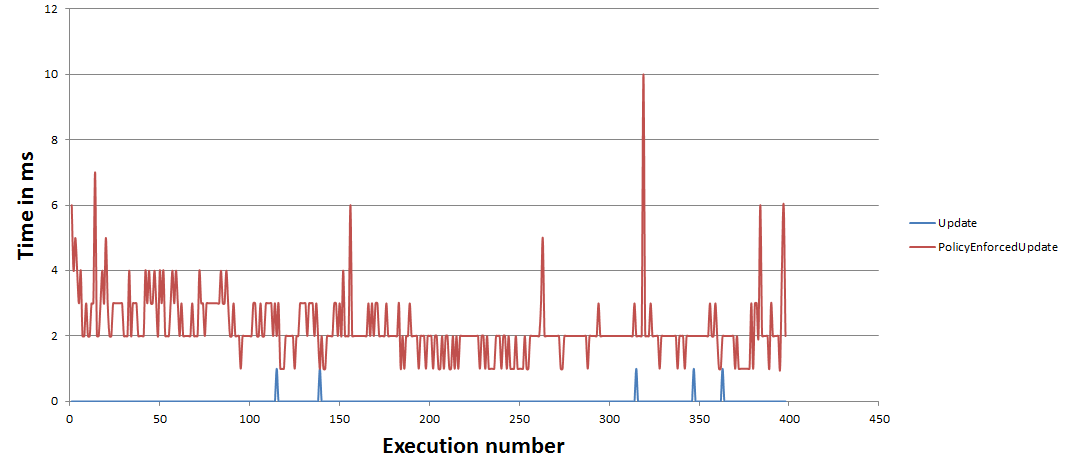
\includegraphics[scale=0.35, trim = 0 0 0 0]{results_update.png}
\caption{Execution times of the laundry machine controller with (PolicyEnforcedUpdate) and without(Update) dynamic policy enforcement over 100 simulations.}
\label{fig:dynamic}
\end{center}
\end{figure}
As we explained in section~\ref{subsec:roles}, the verification is done by the \textit{platform providers}. They release APIs which are used by the third-party manufacturers to develop different types of devices so that they can be integrated to the platforms.  

To explain the analysis, we first give a brief description of how we implemented our smart home simulation. As we saw earlier, there are three types of devices: controllers, sensors and dumb devices. The controllers send commands to the dumb devices depending on the values of one or more sensors. The sensor-controller dependency is implemented as an observer-pattern: the sensors are subjects and controllers are observers. A controller can be the observer of multiple sensors. Whenever a sensor updates the value of a variable (due to change in the value of the parameter it measures), it notifies all its observers. Whenever an observer (controller) is notified, it invokes an \texttt{update()} method inside which it sends a command to a dumb-device, after checking whether the latter can execute the command. This is done by invoking a method: \texttt{checkExecutabilityAndSend(new Command("action\_dumbdevice"))}. 
We verify the following three properties using static analysis:
\begin{enumerate}[topsep=0pt,itemsep=-1ex,partopsep=1ex,parsep=1ex]
    \item A command is sent only within an \texttt{update()} method, i.e. \\
    \texttt{checkExecutabilityAndSend(new Command("action\_dumbdevice"))} is always invoked inside the \texttt{update()} method. This is verified by checking that the latter is the node enclosing the former.
    \item A command is sent only after checking certain conditions inside an \texttt{if-statement}. Similar to the above, this is verified by checking that \texttt{checkExecutabilityAndSend(new Command("action\_dumbdevice"))} is enclosed by an \texttt{if} node.
    \item The clauses in the \texttt{if-statement} are correct according to the policy file of the respective controller. We implemented a dataflow analysis to verify this. Section~\ref{sec:impl} describes this in detail.\\
\end{enumerate}

To further elaborate the analysis, let us consider the example of the smart laundry system. Figure~\ref{fig:policy} shows the dependency policies for the laundry machine controller as defined by a \textit{major organization}, represented in xml format and figure~\ref{fig:code} shows an implementation of the \texttt{update()} method for the laundry machine controller. More than one parameter can be measured by a single sensor. To encode this feature there is a \texttt{class} attribute in the xml file which refers to an instance of a particular sensor.\\

Consider the controller code to be implemented by a \textit{third-party device manufacturer} and given to the \textit{major organization} for integrating to their smart home platform. The latter will first verify the implementation against the specification shown in figure~\ref{fig:policy} and if it is successful, will mark the controller as ``certified" and allow it to be integrated with the platform.\\

\begin{figure}[h]
\begin{center}
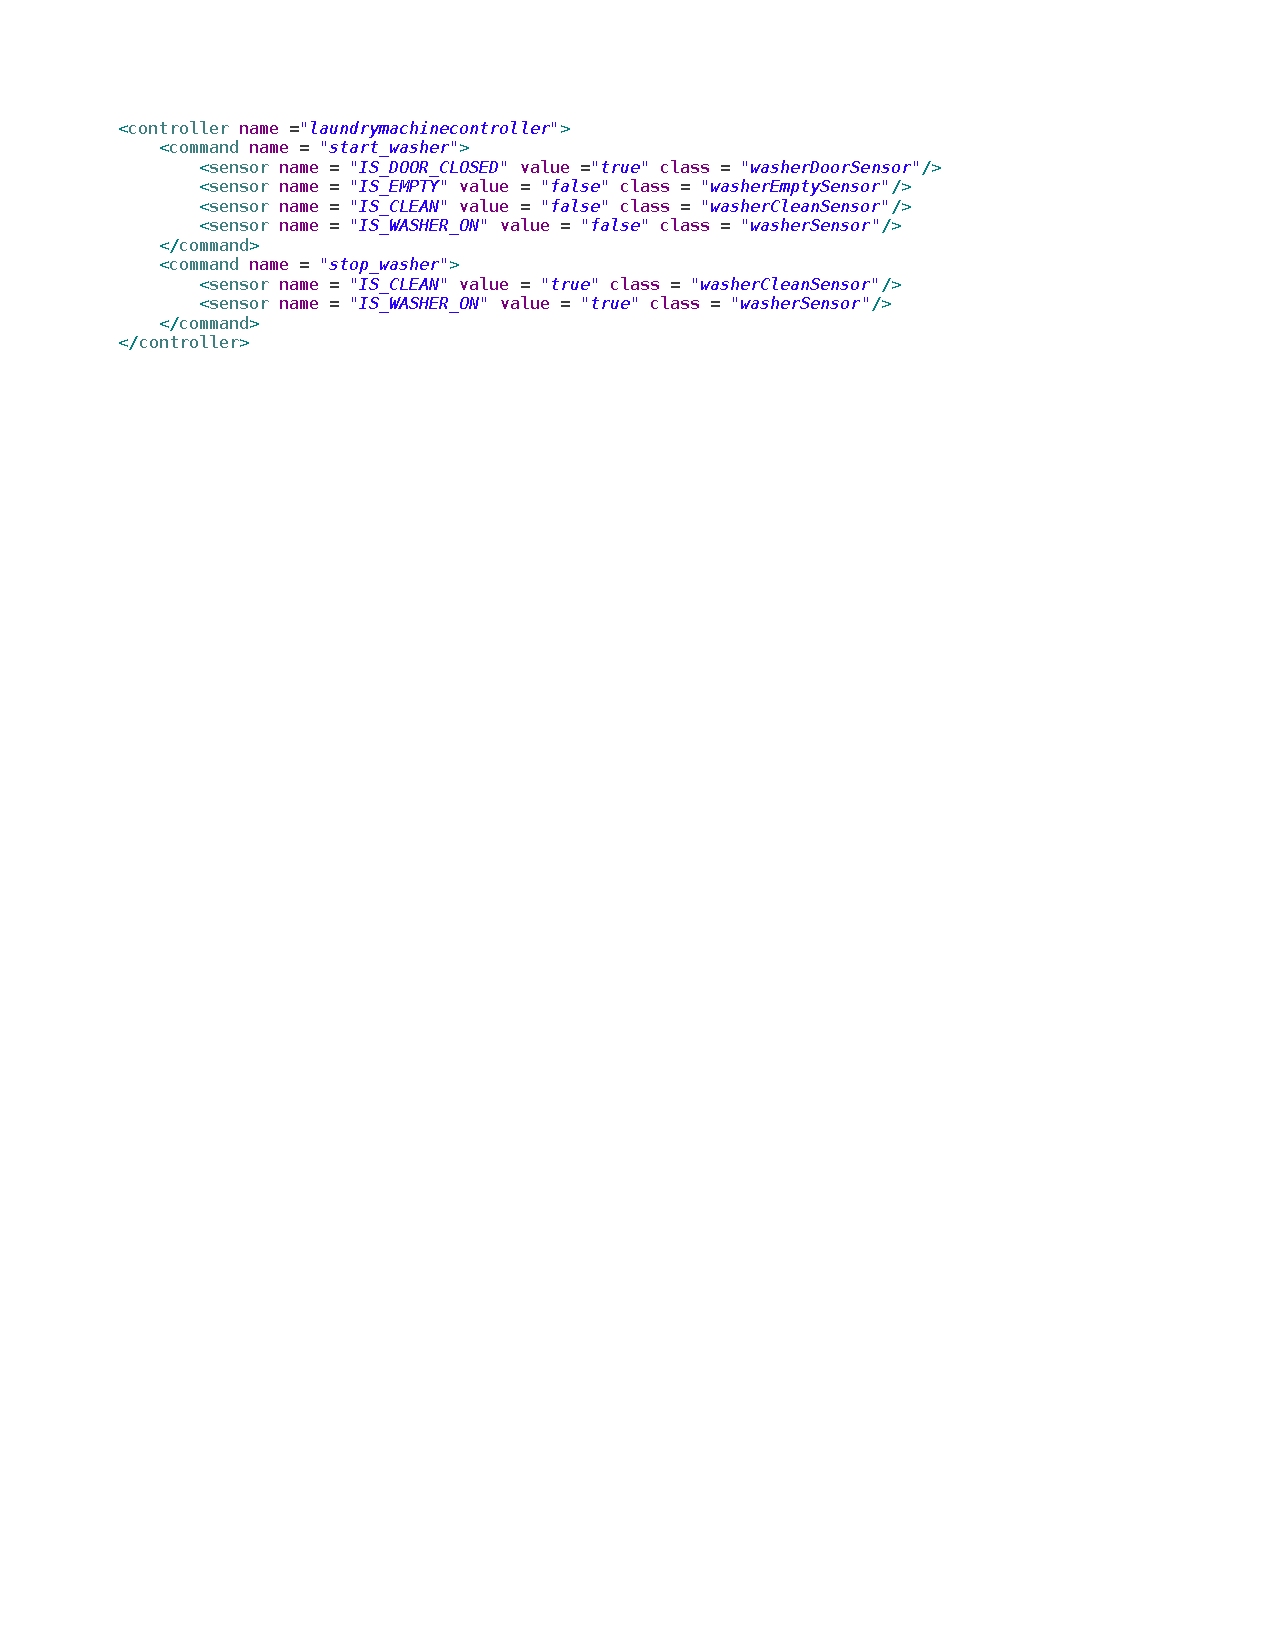
\includegraphics[scale=0.7, trim = 0 21.5cm 0 2cm]{policy.pdf}
\caption{Dependency policies for the laundry machine controller.}
\label{fig:policy}
\end{center}
\end{figure}

\begin{figure}[h]
\begin{center}
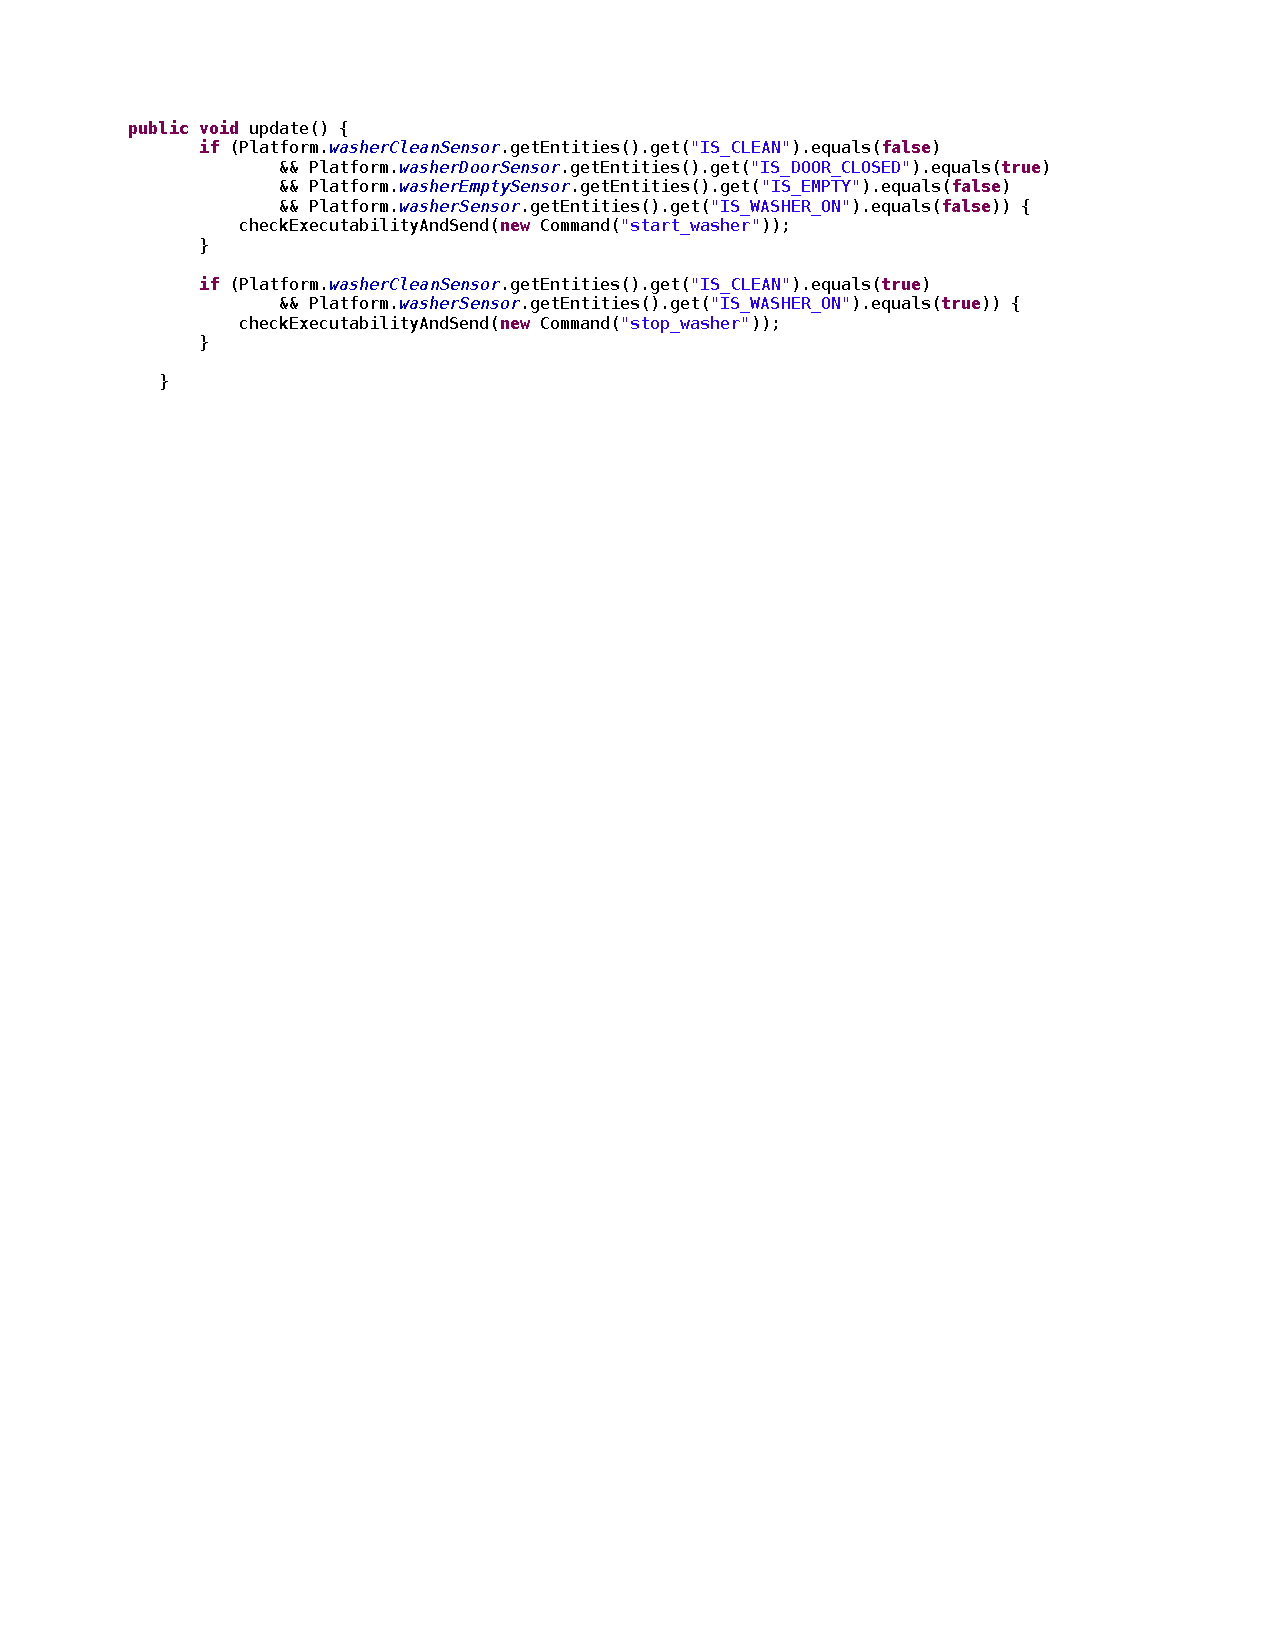
\includegraphics[scale=0.7, trim = 0 21.5cm 0 2cm]{code.pdf}
\caption{\texttt{Update()} for the laundry machine controller. This is a correct implementation which is successfully verified against the policy.}
\label{fig:code}
\end{center}
\end{figure}

\section{Implementation}
\label{sec:impl}
The implementation has two parts: 
\begin{itemize}
\item A simulation of the smart home architecture described in section~\S\ref{sec:archi} together with three smart systems that can be executed on top of it. Table~\ref{table:appliance_sensor} provides a summary of the three smart systems. 
\begin{table*}[h]
\begin{center}
\begin{tabular}{|p{4cm}|p{5cm}|p{4.5cm}|p{3cm}|}
\hline
controller & commands & sensors & \#dependency \newline policies \\ \hline
\tiny{LAUNDRY\_MACHINE\_CONTROLLER} \tiny{ (for dumb device: laundry machine)} &
\small start\_washer, \small stop\_washer & 
\tiny{IS\_WASHER\_ON}, \newline \tiny{IS\_EMPTY, \newline IS\_DOOR\_CLOSED, \newline IS\_CLEANED} & 2\\ \hline


\tiny{GARAGE\_DOOR\_CONTROLLER} \tiny{(for dumb device: garage door)} & 
\small{open\_garagedoor, close\_garagedoor}\tiny &  
\tiny{IS\_GARAGE\_OPEN, \newline IS\_CAR\_INSIDE\_GARAGE, \newline IS\_CAR\_RUNNING, \newline IS\_OWNER\_INSIDE\_CAR,\newline CAR\_DISTANCE (double), \newline CAR\_SPEED (double)} & 4\\ \hline

\tiny{THERMOSTAT} \tiny{(for dumb devices: room heater and air conditioner)} & 
\small start\_roomheater,\newline \small stop\_roomheater,\newline\small start\_airconditioner, \newline \small stop\_airconditioner & 
\tiny{IS\_ROOMHEATER\_ON}, \tiny{IS\_AIRCONDITIONER\_ON},
\tiny{IS\_HOUSE\_EMPTY, \newline IS\_WINDOW\_OPEN, \newline IS\_DOOR\_OPEN, IS\_TEMP\_BELOW\_LOWERTHRESHOLD, IS\_TEMP\_ABOVE\_UPPERTHRESHOLD}, \tiny{OWNER\_DISTANCE (double)} & 8\\ \hline
\end{tabular}
\caption{\small{An example smart home with three smart systems. Each sensor variable has type boolean unless otherwise indicated in parentheses.}}
\label{table:appliance_sensor}
\end{center}
\end{table*}
\item A static analyser that verifies whether the controllers in a smart system comply with their security policy specifications.
\end{itemize}   
From the implementation point of view, we first play the role of a \textit{major organization} and develop the APIs, formalize the specification language, and implement the verification tools. Then we play the role of the \textit{third-party device manufacturers} and develop three smart systems using the APIs. Finally, we again play the role of the \textit{major organization} and verify  the code of the controllers developed by the third parties.

The entire implementation is done in java. The smart home architecture together with the benchmarks (the three smart systems) has approx. 1300 LOC\footref{note1} and the static analyser has approx. 300 LOC\footref{note1}. To simulate the sensors measuring different parameters and updating the corresponding sensor variables, we use pseudorandom number generators in appropriate ranges. \\


We implemented our static analysis tool as a checker on top of Google's error-prone framework~\cite{errorprone}. Error prone is a static analyser for Java and provides an API which can be used to develop different types of program analysis tools. As a part of the static analysis, we also developed a dataflow analysis for verifying the third item mentioned in section~\S\ref{sec:analysis}. The dataflow analyser parses the conditions checked in the \texttt{if-statement} and the statements inside its body to find the command being sent, searches for the policy file (represented in xml format) of the controller, compares the conditions to the policies (sensor values or range of values) in that file, and verifies that the conditions match with those in the policy file for the command being sent inside the body. Figure~\ref{fig:verify1} shows a snippet of the verification code. The verification of the clauses in the \texttt{if-statement} is done inside the \texttt{SEND\_ENCLOSEDBY\_IF} matcher.
\begin{figure}[h]
\begin{center}
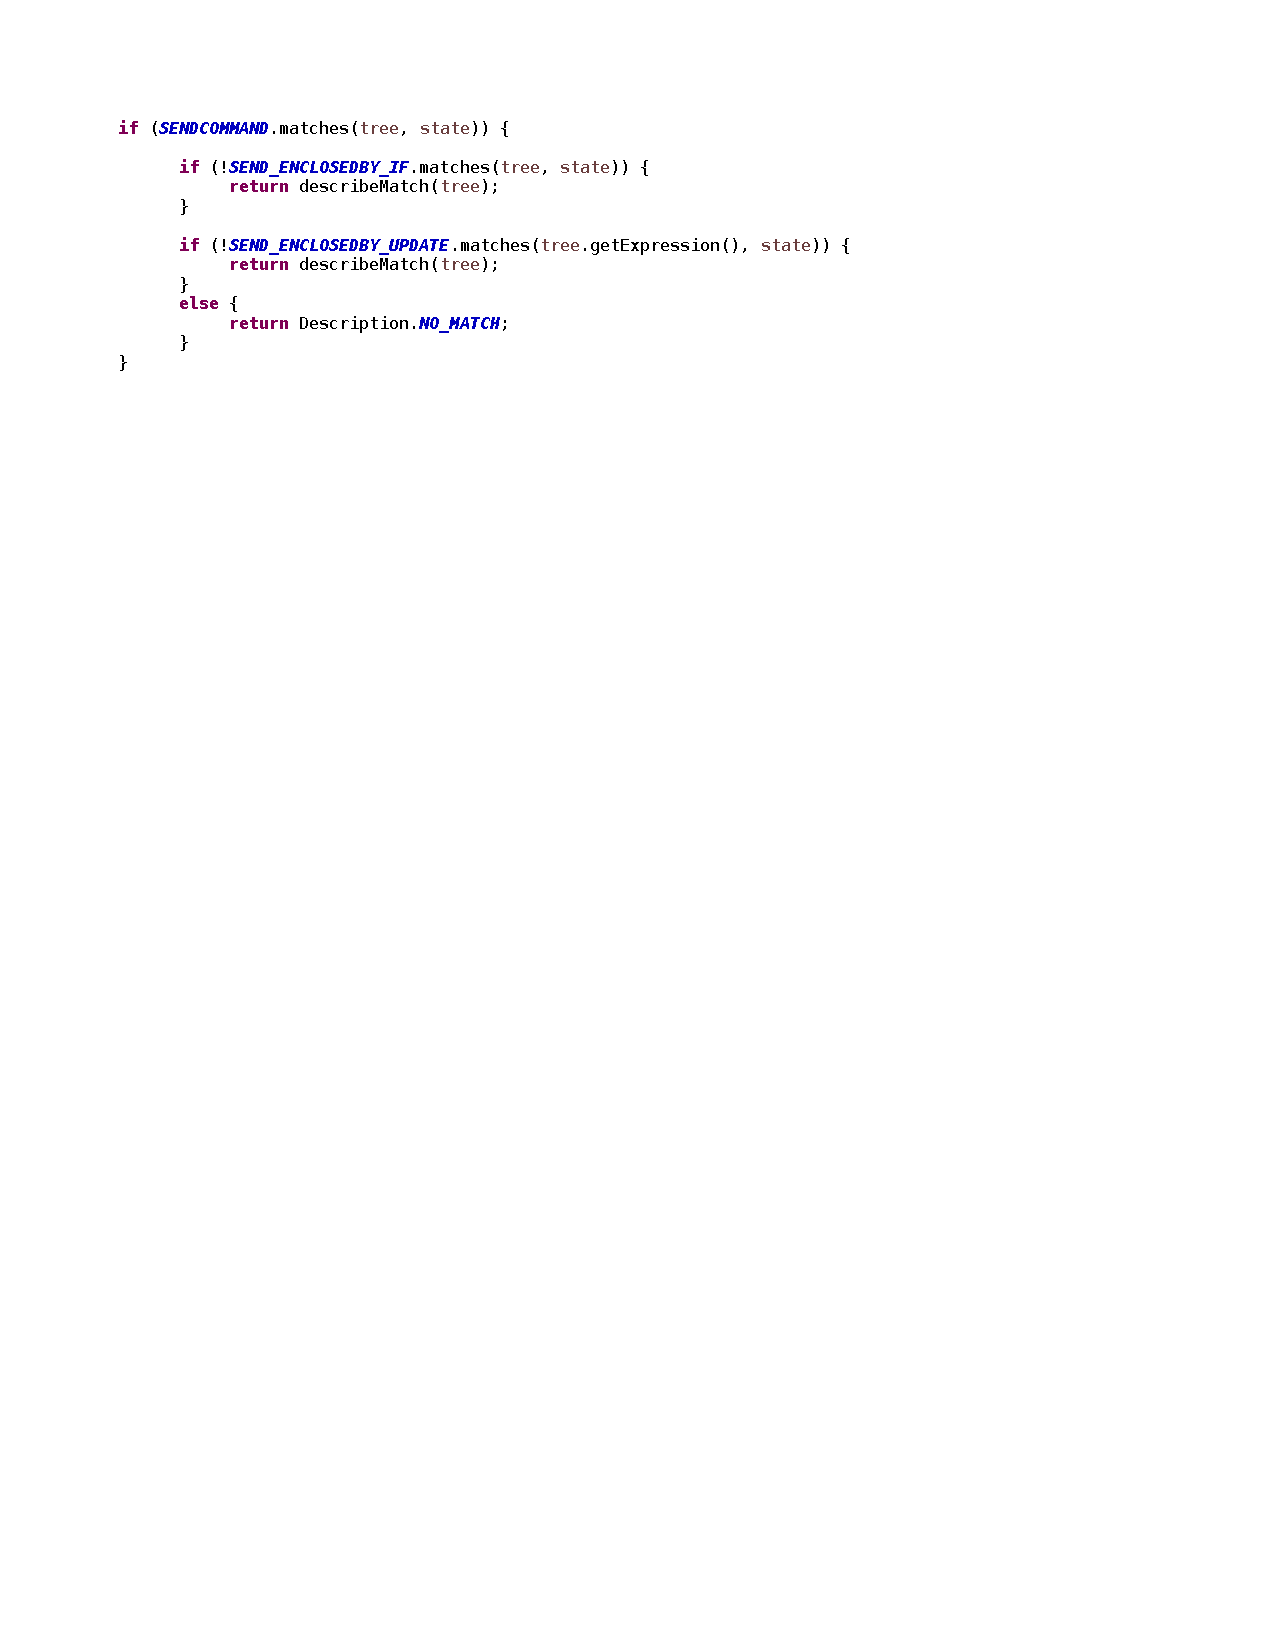
\includegraphics[scale=0.7, trim = 0 22cm 0 2cm]{verify1.pdf}
\caption{Code snippet showing the verification algorithm}
\label{fig:verify1}
\end{center}
\end{figure}


\section{Results}

\section{Conclusions and future work}
In this project, we designed and implemented a simulation of a smart home and developed a static analyser for verifying that the smart systems in the smart home satisfy certain security and correctness policies. We also analysed the various stakeholders in the smart home business and assigned roles to different organizations such that the home owners can have a guarantee that their smart homes are secure. 

We focused only on specifying and verifying the dependency policies for smart homes. As mentioned in section~\S\ref{sec:policies}, there are various other security and correctness policies that are important. As a part of the future work, we plan to verify those other policies and also relax our assumption that the dumb-devices and sensors are trusted. We would also like to extend our prototype to integrate it with some real devices and do an extensive evaluation.
\section{Acknowledgements}
We would like to thank Mike Ernst for his valuable feedback on the ideas and the implementation, and Suzanne Millstein and Konstantin Weitz for their help in figuring out the right tools for doing the verification.
\bibliographystyle{abbrv}
\bibliography{citations}
\end{document}
